\documentclass{beamer}
\usepackage{amssymb,amsthm,amsmath}     % ams
\usepackage[T1]{fontenc}                % skanditavutus
%\usepackage[ansinew]{inputenc}   	% skandien sy�� (windows)
\usepackage[utf8]{inputenc}           % 䤫k�� (linux)
\usepackage[finnish]{babel}       	% suomenkielinen tavutus
%\usepackage{layout}
\usepackage[]{graphicx}
\usepackage{fancyhdr}
\usepackage{amssymb,amsmath,amsthm}
\usepackage{float}
\usepackage{tikz}
\usepackage{siunitx}
\usepackage{physics}
\usepackage{listings}
\usepackage{adjustbox}
\lstset{language=C}
%\pagestyle{fancy}
\linespread{1.24}                      %riviv䬩 1.5
\newcommand{\R}{\mathbb{R}}
\newcommand{\N}{\mathbb{N}}
\newcommand{\Q}{\mathbb{Q}}
\newcommand{\C}{\mathbb{C}}
\begin{document}

\title{computational considerations}
\subtitle{and apparently awesome alliterations}
\author[H]{-}
\frame{\titlepage}
\begin{frame}
\frametitle{what about that quantum}
\framesubtitle{"Quantum mechanics is a trivial theory"\ -Unnamed Instructor}
\begin{align}
\hat{H}_{JC} = \frac{\hbar \Omega}{2}(\hat{a}\hat{\sigma} _+ + \hat{a}^\dagger\hat{\sigma}_-) + \hbar \omega _c \hat{a}^\dagger \hat{a} + \hbar \omega _a \frac{\hat{\sigma}_z}{2}\\
\hat{\sigma}_+ = \ket{g}\bra{e} \\
\hat{\sigma}_- = \ket{e}\bra{g}
\end{align}
stuff in hilbert space = matrices\\
tensor product = matrices\\
everything is matrices
\end{frame}
\begin{frame}
\frametitle{matrices: a solved problem}
\framesubtitle{nice things about matrices}
\begin{itemize}
\item There are numerous libraries available for matrix operations (didn't use them tho)
\item Written by wizards in the 70s (see picture)
\item Run faster than me confronted with the prospect of having to socialize
\end{itemize}
\begin{figure}
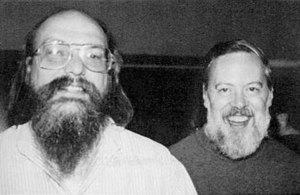
\includegraphics[scale=0.55]{ken.jpg}
\caption{Average numerical linear algebra alpha male}
\end{figure}

\end{frame}

\begin{frame}
\frametitle{matrices: a solved problem}
\framesubtitle{infinite matrices??}
\begin{align}
\hat{a} = \frac{1}{\sqrt{2}} (\hat{x} + i\hat{p})\\
\hat{a}^\dagger = \frac{1}{\sqrt{2}} (\hat{x} - i\hat{p})
\end{align}
matrix rep :
\begin{align}
\hat{a}=\begin{bmatrix}
0 & 1 & 0 & 0 &\hdots \\
0 & 0 & \sqrt{2} & 0 & \hdots\\
0 & 0 & 0 & \sqrt{3}& \hdots \\
\vdots & \vdots & \vdots & \vdots & \ddots
\end{bmatrix}
\end{align}
\end{frame}
\begin{frame}
\frametitle{matrices: a solved problem}
\framesubtitle{truncation and error}
\begin{align*}
\hat{a}=\begin{bmatrix}
0 & 1 & 0 & 0 &\hdots \\
0 & 0 & \sqrt{2} & 0 & \hdots\\
0 & 0 & 0 & \sqrt{3}& \hdots \\
\vdots & \vdots & \vdots & \vdots & \ddots
\end{bmatrix}, \hat{a}^\dagger = \begin{bmatrix}
0 & 0 & 0 & 0 &\hdots \\
1 & 0 & 0& 0 & \hdots\\
0 & \sqrt{2} & 0 & 0& \hdots \\
\vdots & \vdots & \ddots & \vdots & \ddots
\end{bmatrix}
\end{align*}
need to impose a cutoff at some n, but how does error decrease?\\
ERROR = \% OF ELEMENTS THAT DON'T MATCH 
\end{frame}
\begin{frame}
\frametitle{matrices: a solved problem}
\framesubtitle{truncation and error}
\begin{align}
[\hat{a}, \hat{a}^\dagger] = 1
\end{align}
Matrix rep, $n = 5$ and $n = 6$
\begin{align*}
[\hat{a}, \hat{a}^\dagger] = \begin{bmatrix}
1 & 0 & 0 & 0 & 0 \\
0 & 1 & 0 & 0 & 0 \\
0 & 0 & 1 & 0 & 0 \\
0 & 0 & 0 & 1 & 0 \\
0 & 0 & 0 & 0 & 0
\end{bmatrix}, [\hat{a}, \hat{a}^\dagger] = \begin{bmatrix}
1 & 0 & 0 & 0 & 0 & 0\\
0 & 1 & 0 & 0 & 0 & 0\\
0 & 0 & 1 & 0 & 0 & 0\\
0 & 0 & 0 & 1 & 0 & 0\\
0 & 0 & 0 & 0 & 1 & 0\\
0 & 0 & 0 & 0 & 0 & 0
\end{bmatrix}\\
\mathrm{error} = 20\% \ \mathrm{and}\ =18\%
\end{align*}
\end{frame}
\begin{frame}[fragile]
\frametitle{matrices: a solved problem}
\framesubtitle{truncation and error}
so: error decreases as O(n) but matrix size increases as $O(n^2)$.\\

\begin{lstlisting}
for(int i = 0; i < rows; i++) {
	for(int j = 0; j < columns, j++) {
		...
\end{lstlisting}
so execution time: $O(n^2)$, sometimes worse. not ideal, can't be helped!
\end{frame}
\begin{frame}
\frametitle{Why are QM problems computationally difficult?}
\framesubtitle{Computer memory}
computer is a stupid rock tricked in to thinking!\\
memory is aligned, meaning:
\begin{itemize}
\item processor starts reading RAM at addresses divisible by 64(8)
\item 4-byte variables must be in a memory slot divisible by 4, 6 byte variables in spots divisible by 6 etc
\item reading RAM is S L O W
\end{itemize}
\end{frame}
\begin{frame}[fragile]
\frametitle{Why are QM problems computationally difficult?}
\framesubtitle{Computer memory}
illustration:
\begin{lstlisting}
struct Person {
	char first_letter_of_name; // 1 byte
	int age;                   // 4 bytes
	short number_of_kids;      // 2 bytes
}
\end{lstlisting}
\begin{lstlisting}
struct Person {
	char first_letter_of_name; // 1 byte
	char padding[3]            // 3 bytes
	int age;                   // 4 bytes
	short number_of_kids;      // 2 bytes
}
\end{lstlisting}
\end{frame}
\begin{frame}
in code: 7 bytes = single read by CPU\\
in memory: 10 bytes = two reads by CPU = 2x slower!\\
it takes 2-10 ns to access CPU cache, 200+ns to access RAM\\
fix: "memory packing"\ -> reorder the elements according to alignment. NOT POSSIBLE in anything except low level languages\\
QM = huge amounts of data, thus huge amounts of accesses, thus a difficult computational problem
\end{frame}
\begin{frame}[fragile]
\frametitle{Example 1}
\framesubtitle{Semiclassical Rabi}
\begin{align}
\dot{C}_l (t) = -\frac{i}{\hbar}\sum _k C_k(t) \bra{l} H^I \ket{k}
\end{align}
in the code (under the rotating wave approximation):
\begin{lstlisting}
complex double C1 = I/2 *matmul(p,b0,matmul(p,d,k1))
->matrix[0][0]*x2*cexp(I*detuning*t);
complex double C2 = I/2 *matmul(p,b1,matmul(p,d,k0))
->matrix[0][0]*x*cexp(-I*detuning*t);
\end{lstlisting}
\end{frame}
\begin{frame}[fragile]
also, python code to interactively run the simulation:
\begin{lstlisting}[language=python]
import scqo
system = scqo.NLevelAtom(omega = 0.5) 
field = scqo.ClassicalField(omega = 0.5)
system.calculate()
#no rwa
system.set_rwa(False)
system.calculate()
\end{lstlisting}
Plot the results:

\end{frame}
\begin{frame}
lesson about approximations: they might actually suck. cows are not always spherical
\begin{figure}
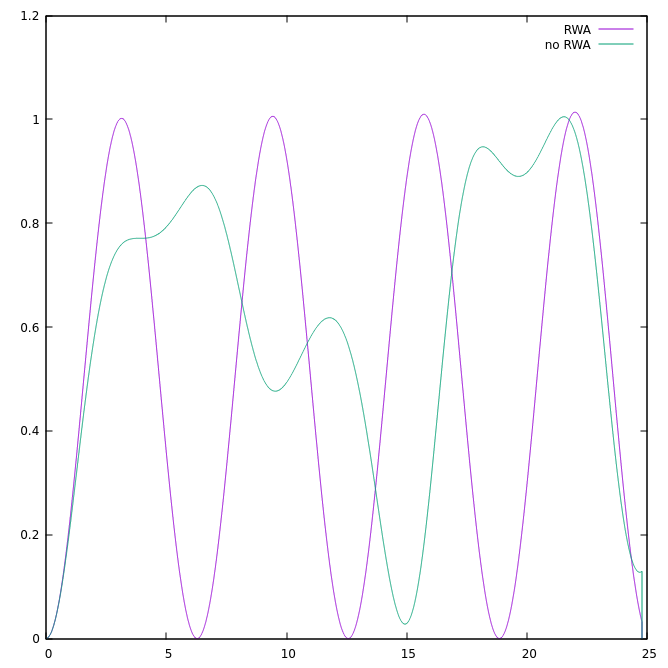
\includegraphics[scale=0.45]{rvsnr.png}
\end{figure}

\end{frame}
\begin{frame}
Different detunings.
\begin{figure}
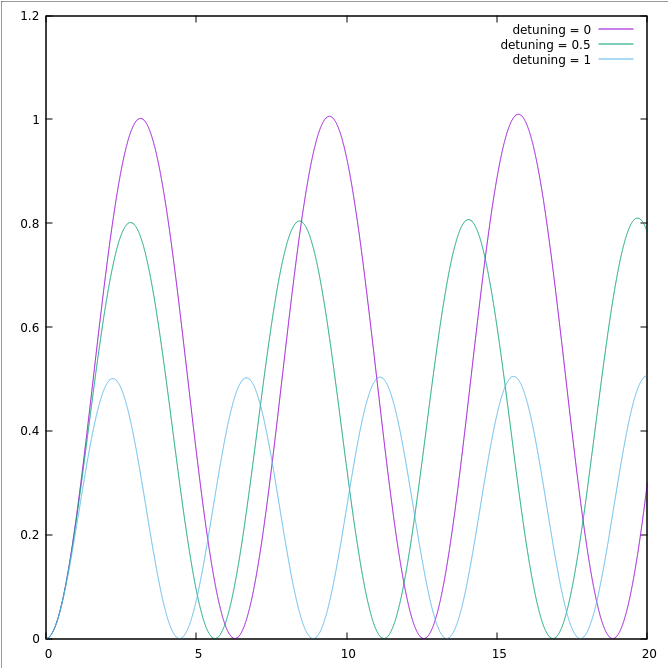
\includegraphics[scale=0.45]{detunings.png}
\end{figure}

\end{frame}
\begin{frame}
..with no RWA
\begin{figure}
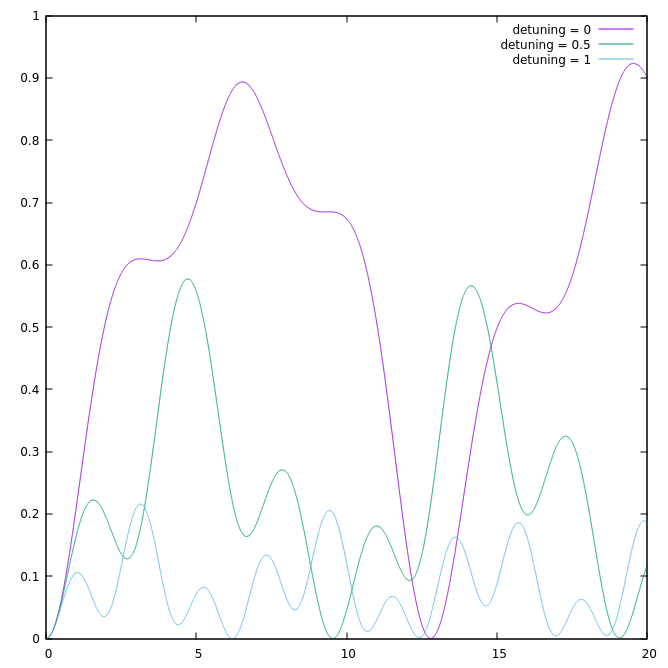
\includegraphics[scale=0.45]{detuningsnorwa.png}
\end{figure}
\end{frame}
\begin{frame}[fragile]
\frametitle{Example 2}
\framesubtitle{Bose-Hubbard dimer (=two sites)}
Bose-Hubbard timer: lattice sites + particles interacting.
\begin{align}
\hat{H} = \epsilon (\hat{a}_1^\dagger \hat{a}_1-\hat{a}_2^\dagger\hat{a}_2) + v (\hat{a}_1^\dagger\hat{a}_2 + \hat{a}_2^\dagger\hat{a}_1) + c(\hat{a}_1^\dagger\hat{a}_1 - \hat{a}_2^\dagger\hat{a}_2)^2
\end{align}
huge matrix size for larger particle numbers, takes forever to run.\\
easy to implement with matrix methods
\end{frame}
\begin{frame}
\frametitle{Example 2}
\framesubtitle{Bose-Hubbard dimer (=two sites)}
\begin{figure}
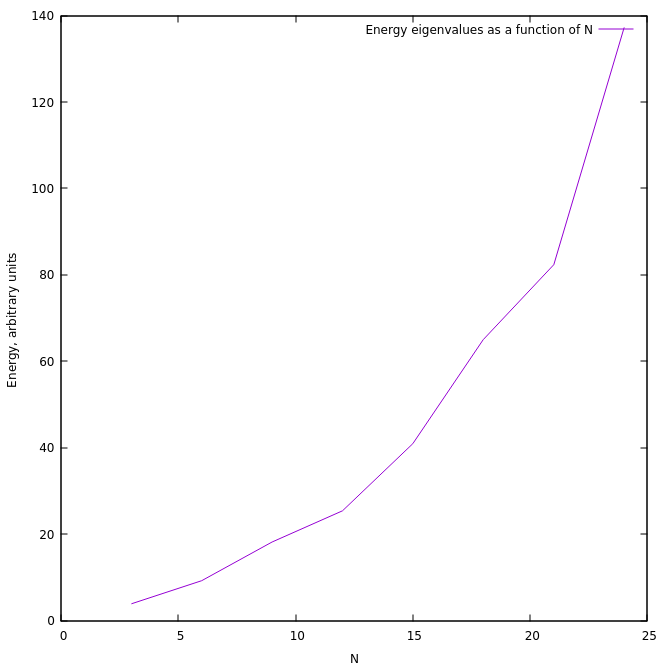
\includegraphics[scale=0.45]{bosehubbard.png}
\end{figure}
\end{frame}
\begin{frame}[fragile]
computational note: you can remove 0-padding from Hamiltonians without losing any important information about the energy levels:
\begin{align}
H = \begin{bmatrix}
0 & 0 & 0 & 0 & 0 & 0\\
0 & a & b & c & d & 0\\
0 & f & b & c & d & 0\\
0 & a & p & q & d & 0\\
0 & a & b & c & d & 0\\
0 & 0 & 0 & 0 & 0 & 0
\end{bmatrix}\iff H = \begin{bmatrix}
a & b & c & d\\
f & b & c & d\\
a & p & q & d\\
a & b & c & d
\end{bmatrix}
\end{align}
Only zeroed eigenvalues are lost, and there are $2n$ of them, where n is the amount of padding removed.
\end{frame}

\begin{frame}
\frametitle{Example 3: Simulating dynamics}
\framesubtitle{Bose-Hubbard Linblad simulation}
The Bose-Hubbard model as an open system (Lindblad form):
\begin{align}
\dot{\hat{\rho}} = -i[\hat{H},\hat{\rho}] - \frac{\gamma}{2}\bigg( \hat{a}_2^\dagger \hat{a}_2 \hat{\rho} + \hat{\rho}\hat{a}_2^\dagger \hat{a}_2-2\hat{a}_2\hat{\rho}\hat{a}_2^\dagger  \bigg)\\
\hat{H} = \epsilon (\hat{a}_1^\dagger \hat{a}_1-\hat{a}_2^\dagger\hat{a}_2) + v (\hat{a}_1^\dagger\hat{a}_2 + \hat{a}_2^\dagger\hat{a}_1) + c(\hat{a}_1^\dagger\hat{a}_1 - \hat{a}_2^\dagger\hat{a}_2)^2
\end{align}
H is the Hamiltonian discussed previously. How about dem dynamics?\\
(optical tunneling from the dimer to optical lattice)
\end{frame}
\begin{frame}
\begin{figure}
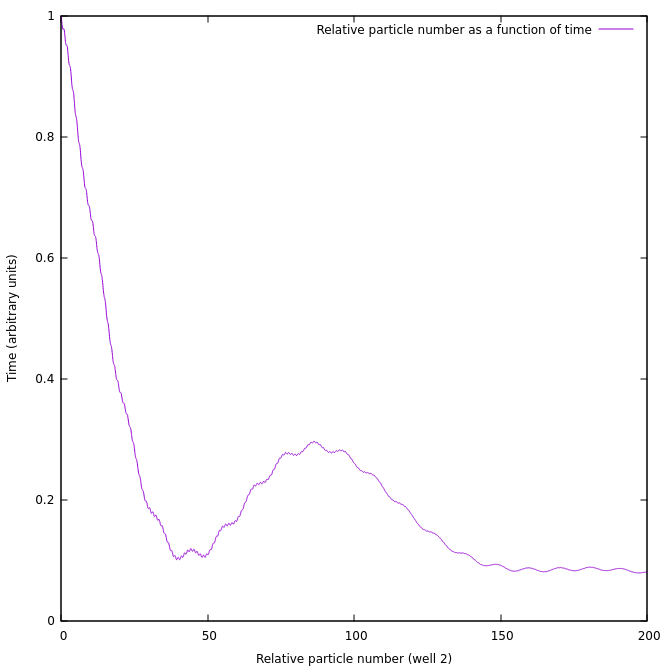
\includegraphics[scale=0.55]{bosehubbardlindblad.png}
\end{figure}
\end{frame}
\begin{frame}
\begin{figure}
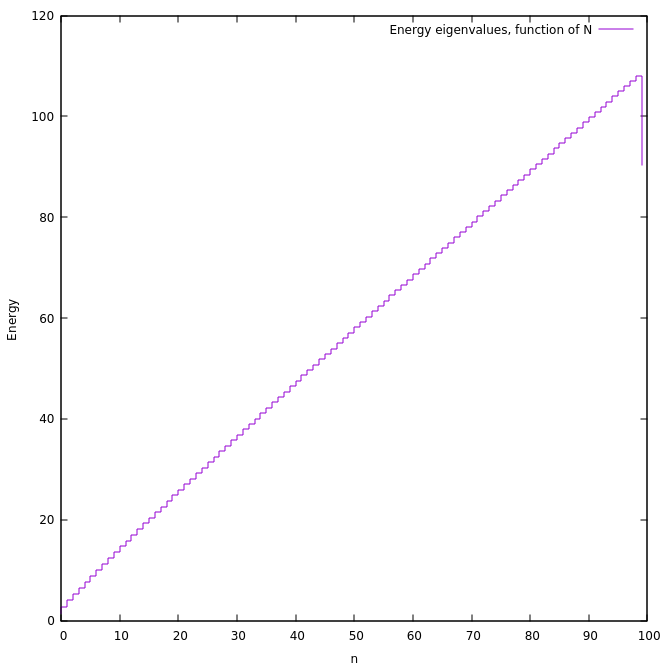
\includegraphics[scale=0.55]{wqc.png}
\end{figure}
\end{frame}
\begin{frame}
\frametitle{Some conclusions}
\begin{itemize}
\item Matrices are a straightforward way of doing OQS
\item The method is a bit slow (could be heavily optimized)
\item Special care is needed to choose the right algorithms for unstable problems
\item Approximations sometimes suck
\item I hate segfaults
\end{itemize}
\end{frame}
\end{document}